{\let\clearpage\relax\let\cleardoublepage\relax
\chapter{Disco protoplanetario}
}


Il materiale presente nella regione instabile di una nube molecolare \'e dotato di momento angolare quindi accresce sulla massa della protostella centrale formando un disco ortogonale al momento totale della nube che trascurando l'effetto della pressione del gas, ruota con velocit\'a angolare kepleriana.

%Jansky=10-23erg/(s*cm2*Hz)
\begin{workout}[Refs dischi protoplanetari]
Chronology of  early stages: apai lauretta 10 (book)
\end{workout}

\section{Modello disco di accrescimento}

Nei modelli unidimensionali per disco di accrescimento si descrive il trasporto di momento angolare verso l'esterno introducendo la viscosit\'a aumentata $\nu=\frac{\eta}{\rho}\to\alpha c_s H$: giustifico euristicamente la parametrizzazione della viscosit\'a del disco di accrescimento in analogia alla viscosit\'a molecolare (\cite{bouvier2002theory}).

\begin{workout}[Strees tensor]
appendix a pg 66 planet formation and migration vs crida PHD torque calculation pg 24
\end{workout}
\begin{workout}[Stress tensor in keplerian disk: crida PHD]
pg 26
\begin{align}
&\sigma_{ij}=d_{ij}-PI{ij}\\
&d_{ij}=2\Sigma\nu(D_{ij}-\frac{1}{3}(\div{\vec{v}}I_{ij})+\Sigma\zeta(\div{\vec{v}})I_{ij}\\
&D_{ij}=\frac{1}{2}(\partial_iv_k+\partial_kv_i)
\end{align}
\end{workout}

L'equazione del moto per un elemento di fluido \'e
\begin{align}
&\PDof{t}(\rho v_i)+\PDof{x_i}(\rho v_iv_j+T_{ij})=F_i\label{eq:fluidmotion}\\
&T_{ij}=P\delta_{ij}-\sigma_{ij}\\
&\sigma_{ij}=\eta(\partial_jv_i+\partial_iv_j-\frac{2}{3}\delta_{ij}\partial_kv_k)+\zeta\delta_{ij}\partial_kv_k
\end{align}
dove $\eta$, $\zeta$ sono le shear e bulk viscosity, quest'ultima legata ai gradi di libert\'a interni della molecola \'e trascurabile se i tempi di equipartizione interni sono molto minori del tempo fra due collisioni.
%-$\sigma_{ij}$ \'e flusso di componente i di momento in direzione j
Considero la velocit\'a istantanea di una molecola nel piano xy $(v_x+u_x,u_y)$, dove u \'e la componente casuale e $\exv{}$ rappresenta media temporale (agitazione termica: $\exv{u}=0$) quindi
\begin{equation}
\sigma_{xy}=-\rho\exv{u_xu_y}
\end{equation}

D'altra parte la forza viscosa agente sulla molecola \'e
\begin{equation}
F_{visc,x}=\TDy{y}{\sigma_{xy}}\approx\TDof{y}(\eta\TDy{y}{v_x})
\end{equation}
%PRIM'ORDINE IN \lambda/L
Dalle equazioni precedenti si ha che
\begin{equation}
\exv{u_iu_j}=-\nu\TDy{x_j}{v_i}\label{eq:molvisccorr}
\end{equation}
%con $\eta=\rho\nu$.

Per un disco di densit\'a superficiale $\Sigma(r,t)$, dotato del campo di velocit\'a $(v_r,v_{\phi})=(u_r,r\Omega+u_{\phi})$, scrivo le equazioni di conservazione di massa e la componente azimutale dell'equazione del moto
\begin{align}
&\PDy{t}{\Sigma}+\frac{1}{r}\PDof{r}(r\Sigma v_r)=0\label{eq:massconservation}\\
&\Sigma(\PDy{t}{v_{\phi}}+v_r\PDy{r}{v_{\phi}}+\frac{v_rv_{\phi}}{r})=0
\end{align}

Dalle equazioni precedenti segue l'equazione del momento angolare:
\begin{equation}
\PDof{t}[r\Sigma(r\Omega+u_{\phi})]+\frac{1}{r}\PDof{r}[r^2\Sigma(r\Omega+u_{\phi})u_r]=0
\end{equation}
Trascuro la fluttuazione azimutale nel termine di derivata temporale e considero media spaziale su scala opportuna:
\begin{equation}
\PDof{t}r^2\Sigma\Omega+\frac{1}{r}\PDof{r}[r^3\Sigma\Omega\exv{u_r}+\Sigma r^2\exv{u_ru_{\phi}}]=0\label{eq:smoothedangularmomentumequation}
\end{equation}
%\vec{v}=(u_r,\Omega r)
In analogia all'equazione \eqref{eq:molvisccorr} si definisce
\begin{equation}
\sigma_{r\phi}=-\Sigma\exv{u_ru_{\phi}}=\Sigma\nu r \TDy{r}{\Omega}
\end{equation}

\begin{wrapfigure}[17]{l}{0.5\textwidth}
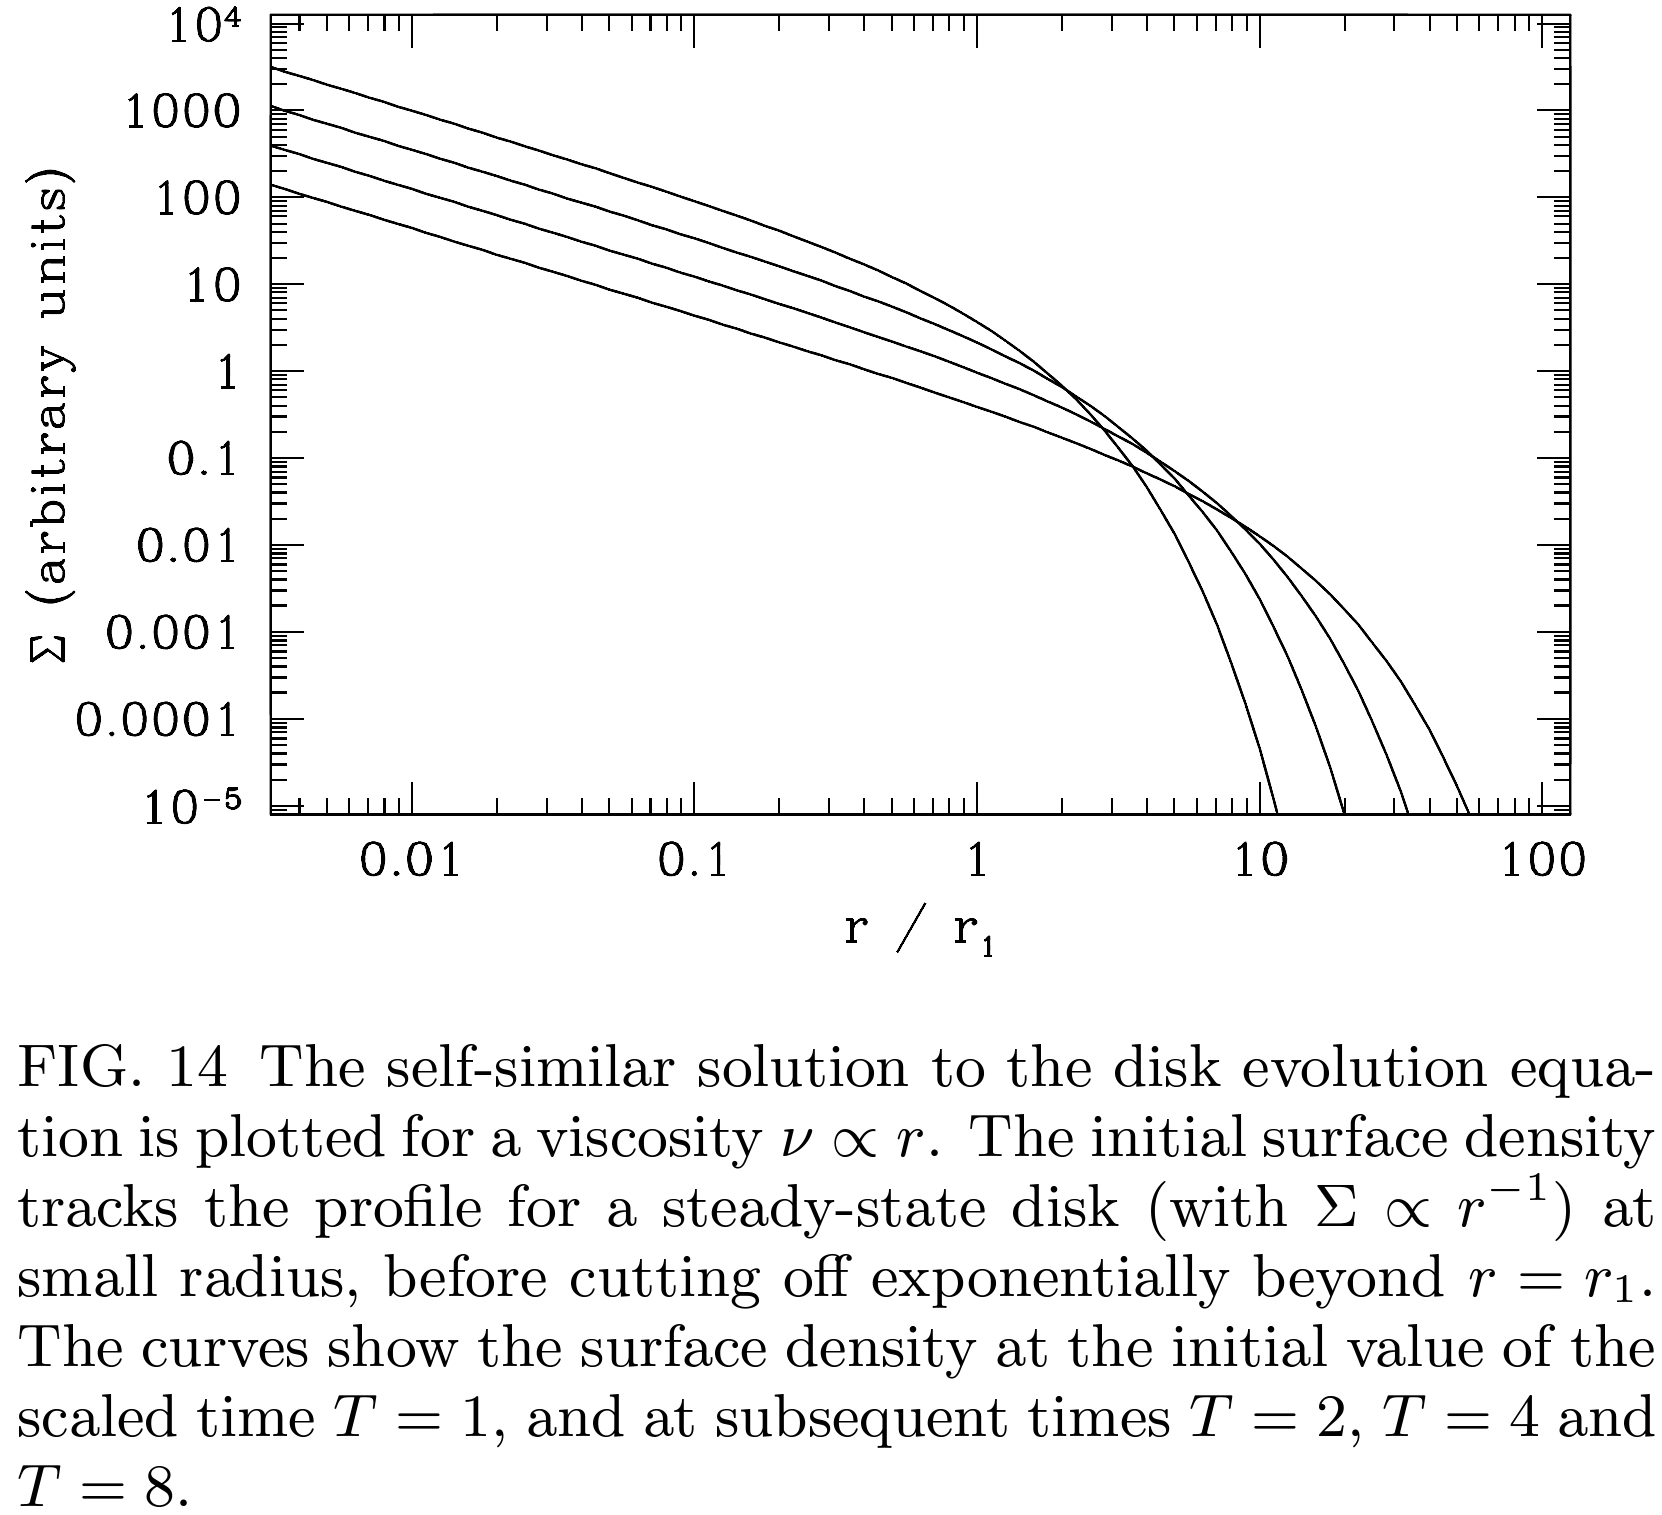
\includegraphics[trim={0cm 19cm 0 0},clip, keepaspectratio,width=0.48\textwidth]{selfsimilaralphadisk}
\caption{Soluzione equazione \eqref{eq:sigmaevol} per $\nu\propto r\expy{\gamma}$ con $\gamma=1$. Da \cite{armitage2007lecture}.}\label{fig:selfsimilaralphadisk}
\end{wrapfigure}

Nei modelli di disco di accrescimento unidimensionali si parametrizza il trasporto di momento angolare ponendo
\begin{equation}
\nu=\alpha c_s H
\end{equation}
dove $\alpha$ \'e parametro da fissare, $c_s$ la velocit\'a del suono e H lo spessore del disco. Utilizzo l'equazione di conservazione della massa per riscrivere \eqref{eq:smoothedangularmomentumequation}:
\begin{equation}
\PDy{t}{\Sigma}=3\frac{1}{r}\PDof{r}[r\expy{1/2}\PDof{r}(\nu\Sigma r\expy{1/2})]\label{eq:sigmaevol}
\end{equation}

La struttura verticale \'e determinata dalla componente lungo z dell'attrazione del corpo centrale
%profilo termico determinato da equilibrio termico
\begin{equation}
\TDy{z}{P}=-\rho g_z=-\frac{GM_*}{r^2+z^2}\frac{z}{r}\rho=-\Omega^2\rho z
\end{equation}
mentre la struttura radiale del disco di gas \'e determinata dall'equilibrio idrostatico
\begin{equation}
\frac{v_g^2}{r}=\frac{GM_*}{r^2}+\frac{1}{\rho}\TDy{r}{P}
\end{equation}
dove ho introdotto $v_g$ velocit\'a a cui il gas orbita attorno alla stella centrale.

\begin{figure}[!ht]
\begin{subfigure}[b]{0.39\textwidth}
\centering
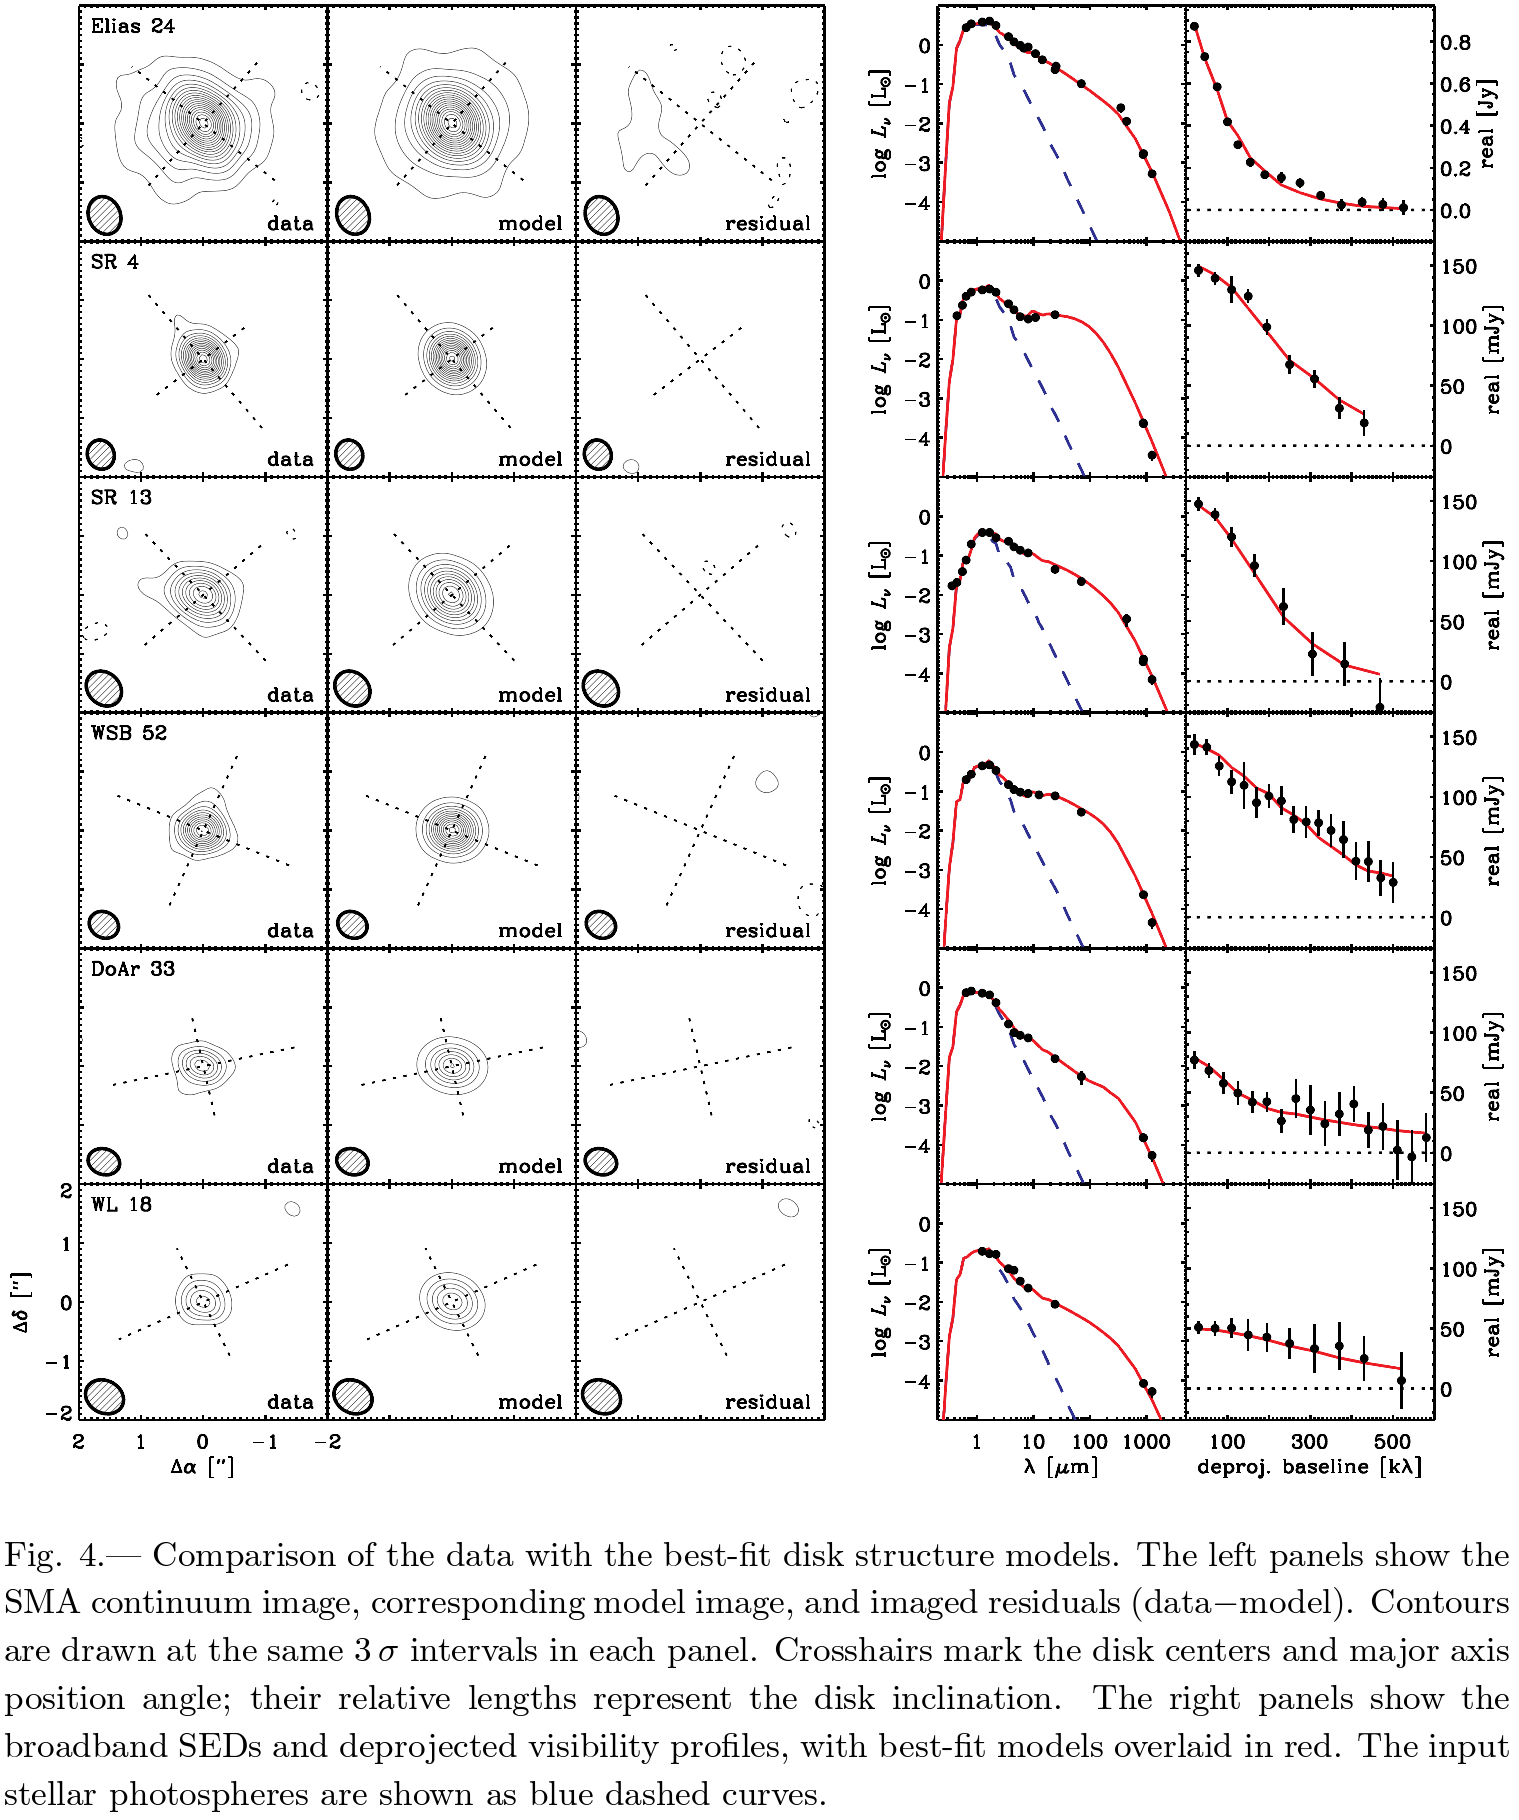
\includegraphics[trim={0cm 10cm 0 0},clip, keepaspectratio,width=0.98\textwidth]{SED-contours}
\caption{Struttura dischi protoplanetari (flusso a $\lambda=\SI{880}{\micro\meter}$) e densit\'a spettrale. La linea tratteggiata viola indica la distribuzione di corpo nero della fotosfera stellare. Da \cite{andrews2010protoplanetary}.}\label{fig:SED-contours}
\end{subfigure}
~
\begin{subfigure}[b]{0.55\textwidth}
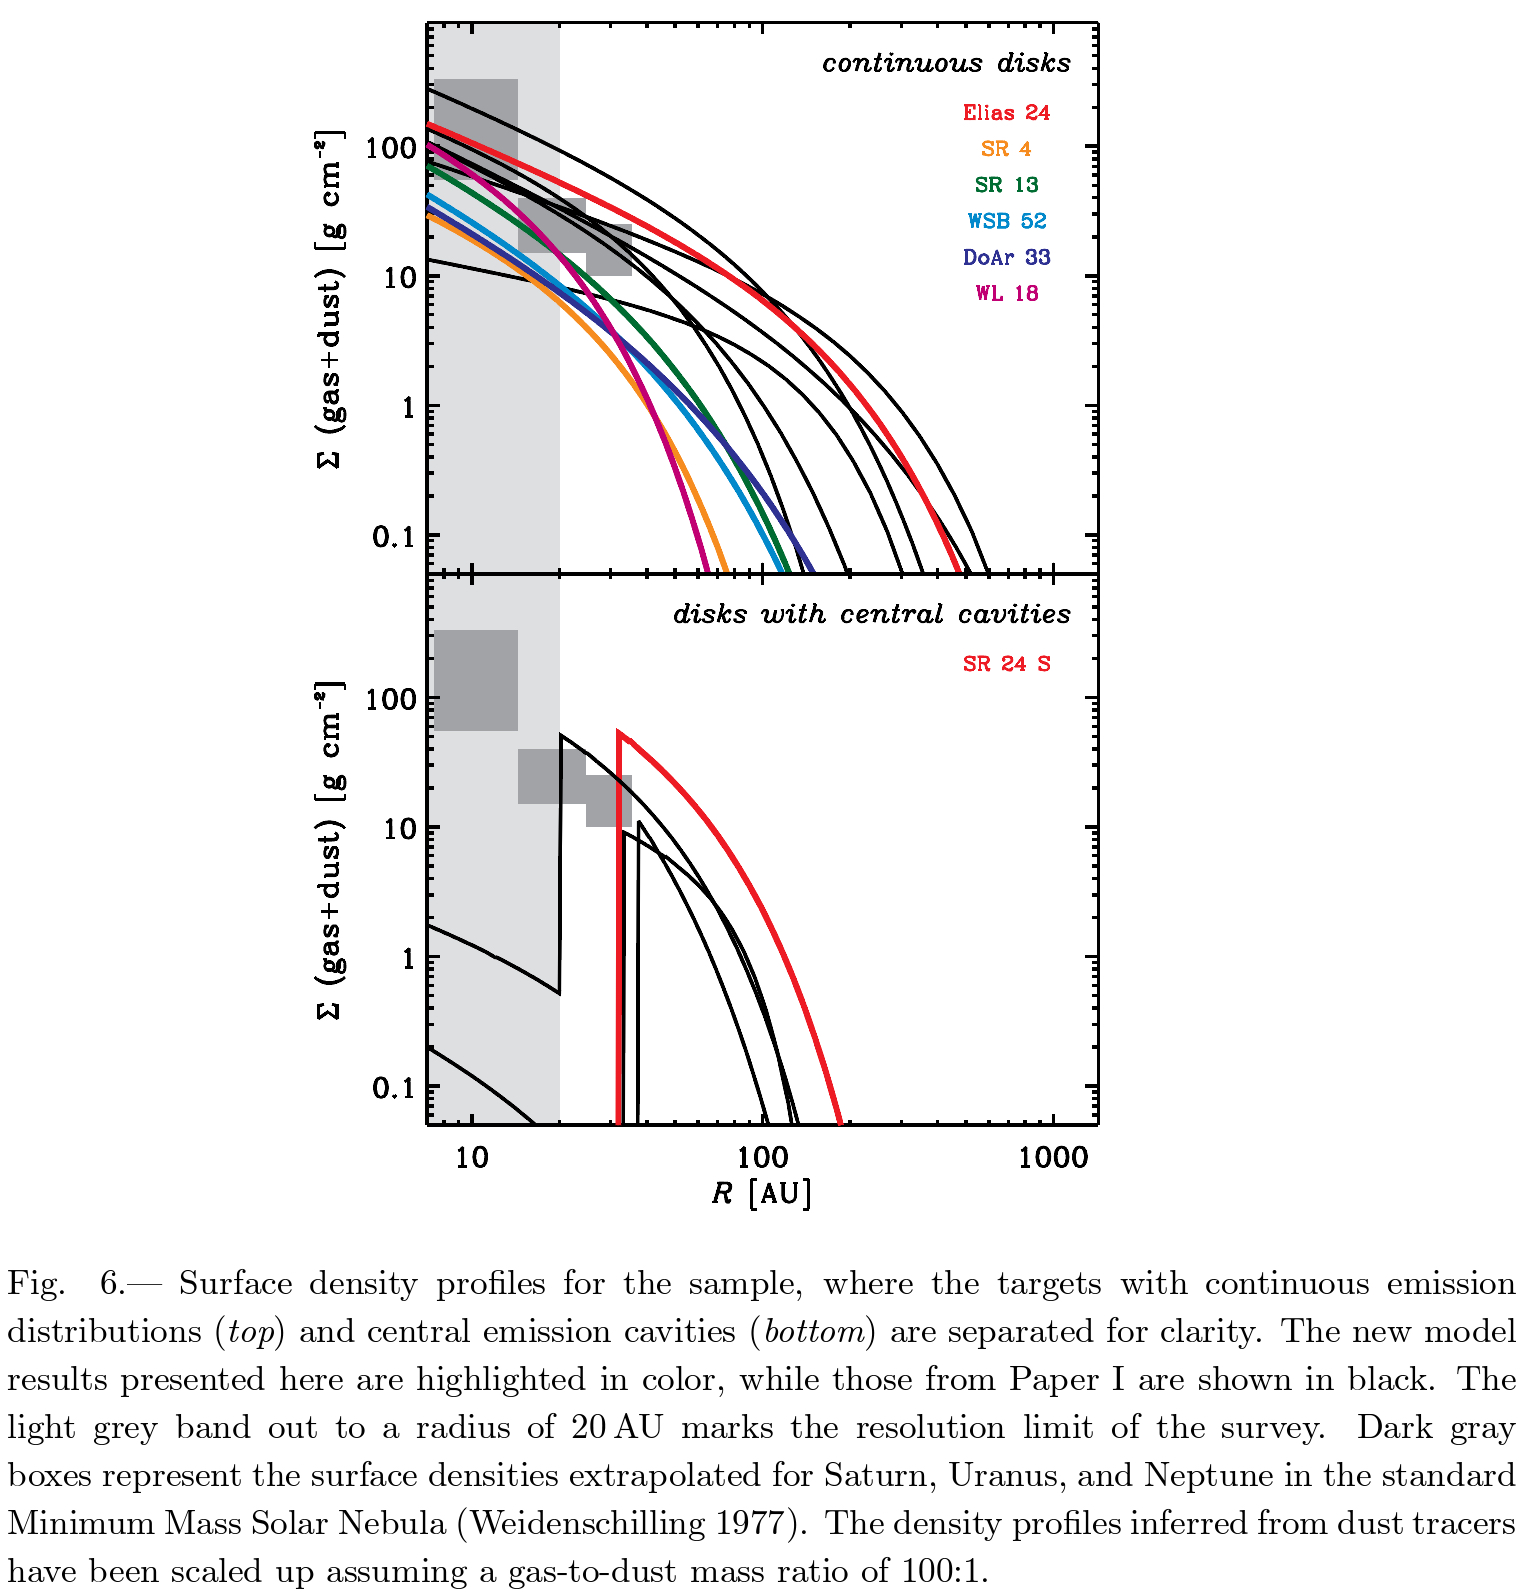
\includegraphics[trim={0cm 15cm 0 0},clip, keepaspectratio,width=0.98\textwidth]{diskdensity}
\caption{Densit\'a superficiale dischi protoplanetari osservati nella regione di Ophiuchus ricavata risolvendo modello disco di accrescimento che riproduca densit\'a spettrale di energia osservata. I rettangoli grigi indicano densit\'a superficiale per la MMSN nella regione di Saturno, Urano e Nettuno. Da \cite{andrews2010protoplanetary}.}\label{fig:diskdensity}
\end{subfigure}
\end{figure}

Attorno alle stelle giovani sovente si trovano strutture opache nel visibile ma otticamente sottili nelle onde infrarosse: risolvendo il modello di disco protoplanetario, avente come input la distribuzione della dimensione della polvere e rapporto gas/polvere, per riprodurre le caratteristiche spettrali e flusso termico osservati, note anche le caratteristiche della stella centrale, si determinano i parametri caratteristici del disco.

La figura (\subref{fig:SED-contours}) mostra le strutture attorno a stelle giovani del cluster Ophiuchus secondo profili di intensit\'a a \SI{880}{\micro\meter}. Se $\nu\propto r\expy{\gamma}$ una soluzione di \eqref{eq:sigmaevol} per $t=0$ \'e
\begin{equation}
\Sigma=(2-\gamma)\frac{M_d}{2\pi R_c^2}(\frac{r}{R_c})\expy{-\gamma}\Exp{-(\frac{r}{R_c})\expy{2-\gamma}}
\end{equation}
\cite{andrews2010protoplanetary} hanno osservato lo spettro emesso da oggetti nella regione di formazione stellare Ophiuchus determinando massa, dimensioni caratteristiche e viscosit\'a: $M_d=0.004-0.143\msun{}$, $\gamma=0.4-1.1$, $R_c=\SIrange{14}{198}{\astronomicalunit}$.

\begin{wrapfigure}[6]{l}{0.5\textwidth}
\centering
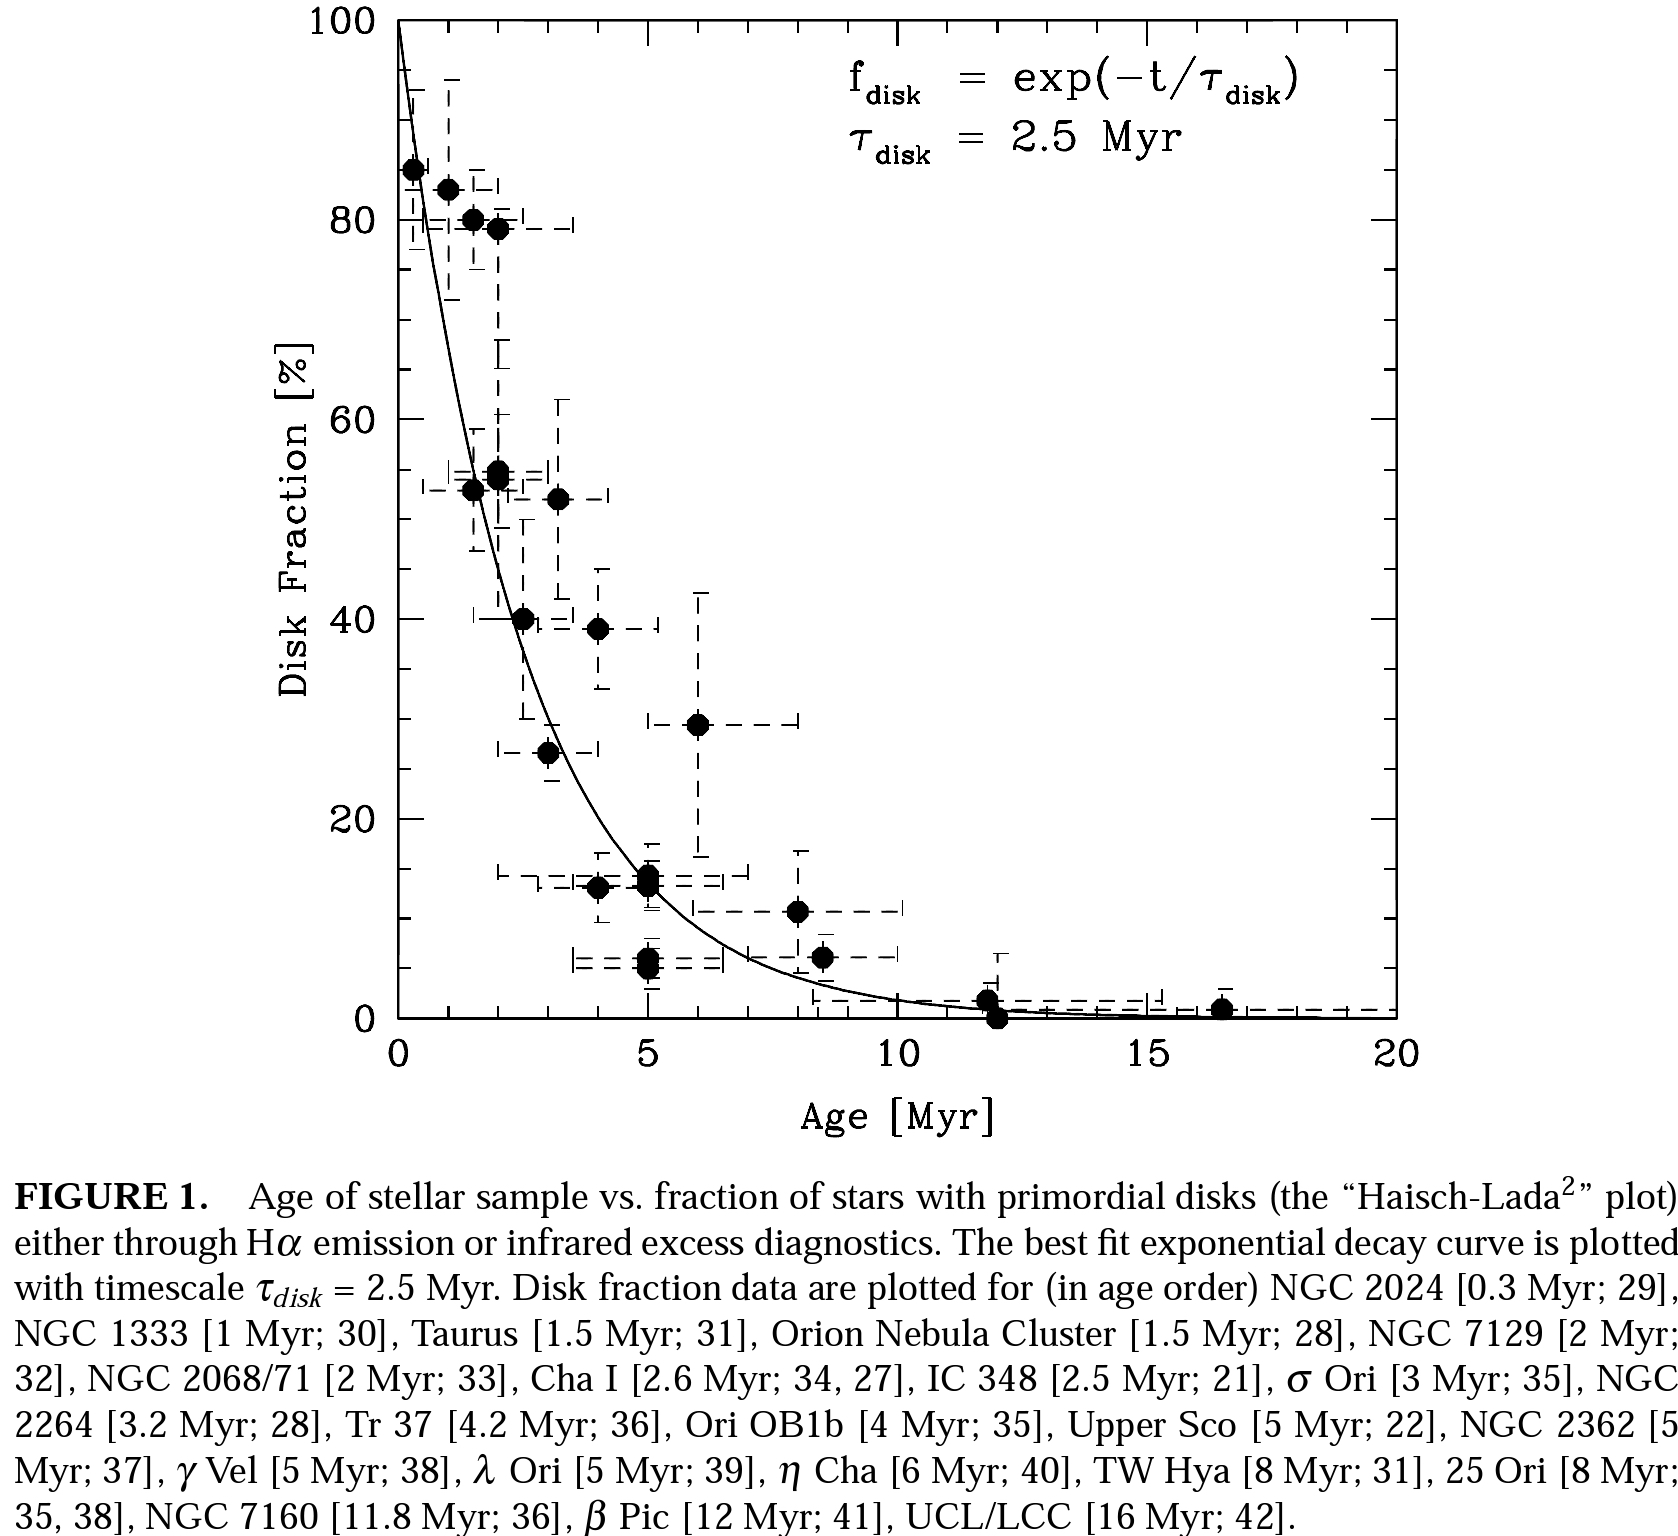
\includegraphics[trim={0cm 13cm 0 0},clip, width=0.49\textwidth,keepaspectratio]{clusterage-fstar}
\caption{Frazione di stelle con disco protoplanetario in funzione dell'et\'a del cluster. Da \cite{mamajek2009initial}. }\label{fig:clusterage-fstar}
\end{wrapfigure}

In figura (\ref{fig:clusterage-fstar}) \'e riportata la sfrazione di stelle con dischi protoplanetari in funzione dell'et\'a del cluster. \'E possibile stimare tempo di vita caratteristico del disco considerando andamento esponenziale per frazione di dischi: secondo (\cite{mamajek2009initial}) $\tau_c\approx\SI{2.5}{\mega\year}$, mentre (\cite{haisch2001disk}) hanno determinato $\tau_c\approx\SI{6}{\mega\year}$.

\vspace{0.2\textheight}

\begin{workout}[Caratteristiche fittate proto-dischi]
\begin{table}[!ht]
\begin{tabular}{|ccccc|}
Nome&$M_d$&$\gamma$&$R_c$&$H_{100}\\
AS 205&0.029&0.9&46&19.6&0.11
\end{tabular}
\end{table}
\end{workout}

\begin{workout}[Profilo densit\'a verticale disco isotermo]
Thin vertically isothermal disk
\begin{align}
&\rho(z)=\frac{\Sigma}{h\sqrt{2\pi}}\exp{-\frac{z^2}{2h^2}}
&
\end{align}
\end{workout}

\begin{workout}[Profilo termico del disco]

\end{workout}

\begin{workout}[Momento torcente in disco Kepleriano]
\begin{align}
&\sigma_{ij}=2\Sigma\nu D_{ij}=\Sigma\nu\begin{pmatrix}0&-\Omega\partial_r(r\Omega)\\-\Omega+\partial_r(r\Omega)&0
\end{pmatrix}\\
\end{align}
Il momento torcente esercitato da S su $C^c$ \'e
\begin{equation}
T=\iint_{S^c}(\vec{r}\wedge\nabla\sigma)\,ds=\int_S\vec{r}\wedge(\sigma\,dl\vec{n})
\end{equation}
Nel caso S sia circonferenza di raggio r:
\begin{equation}
T_{\nu}=3\pi r^2\Omega_0\Sigma\nu
\end{equation}
\end{workout}

\begin{workout}[Passive disks]
(Refs: Ref: spectral energy distribution of T-Tauri star with passive circumstellar disk)
Dust passively reirradiate star light
\end{workout}

\begin{workout}[Struttura verticale del disco, profilo termico]
Pressione gas determinata da equilibrio idrostatico
\end{workout}

\begin{workout}[Viscous/turbulent disk]
laminar (high momentum diffusion)
mass inflow Gullbring98 \SIrange{e-9}{e-7}{\per\year}$\msun{}$
\end{workout}
\begin{workout}[MRI]
fig 10.3:
gammie 1996
\end{workout}

\begin{workout}[alpha prescription]
$\vec{v}=(u_r,r\Omega)$, stress tensor $\sigma_{r\phi}=-\Sigma\exv{u_ru_{\phi}}$.
Enhanced turbulent viscosity: $-\Sigma\exv{u_ru_{\phi}}=\Sigma\nu r\TDy{r}{\Omega}$, $\nu=v_TH$, $\alpha=v_T/c_s$
\end{workout}

\begin{workout}[Accretion disk sources]
Lodato: classical disk physics
o218, 296: disk formation, constrains from solar system
the alpha disk pg 18: theory of turbulent accretion disk
\end{workout}

\begin{workout}[Isothermal cloud collapse!]

\end{workout}

\begin{workout}[Descrizione trasporto momento angolare tramite parametrizzazione viscosit\'a]
Mass conservation + momentum conservation in viscous flow: angular momentum evolution. Phenomena: Shear viscosity - turbulence - MRI.
Nei modelli 1D per disco di accrescimento si parametrizza viscosit\'a tramite $\nu=\frac{\eta}{\rho}\to\alpha c_s H$: la viscosit\'a molecolare \'e troppo bassa  per trasportare all'esterno il momento angolare sui tempi-scala osservati.
Theory of turbulent accretion disk: pg 18, 8.
Flusso di x-momentum lungo y $\rho\exv{u_xu_y}$, dove considero la velocit\'a dell'elemento di fluido $(v_x+u_x,u_y)$ dove le $u$ rappresentano fluttuazioni della velocit\'a: $\sigma_{xy}=-\rho\exv{u_xu_y}$.
Ricordando la definizione di tensore degli stress e con $\vec{v}=v_x(y)\hat{x}$
\begin{equation}
\sigma_{ij}=\eta(\partial_jv_i+\partial_iv_j-\frac{2}{3}\delta_{ij}\partial_kv_k+\zeta\delta_{ij}\partial_kv_k \to \eta\TDy{y}{v_x}
\end{equation}
\begin{equation}
\PDof{t}(\rho v_i)+\PDof{x_i}(\rho v_iv_j+T_{ij})=F_i
\end{equation}
Fluttuazioni: $\sigma_{ij}=-\rho\exv{u_iu_j}$.
Viscosit\'a molecolare: $\exv{u_iu_j}=-\nu\TDy{x_j}{v_i}$.
Turbulence: Reynpold stress $\tau_{ij}=-\rho\exv{v_jv_i}$, $\exv{u_iu_j}=-\nu_T\TDy{x_j}{v_i}$
\begin{equation}
\PDy{t}{\Sigma}=3\frac{1}{r}\PDof{r}[r\expy{1/2}\PDof{r}(\nu\Sigma r\expy{1/2})]
\end{equation}
\end{workout}

\begin{workout}[Photoievaporation: X-EUV-FUV (Alexander13: The Dispersal of Protoplanetary Disks)]
Protoplanetary disc evolution and dispersal: the implications of X-ray photoevaporation.
\end{workout}


\begin{workout}[Foto-evaporazione]
(Photoevaporation: veras armitage 2003, Alexander13, Mordasini12. Internal/External).
EUV($E\approx13.6eV$): ionization, FUV($E\approx6-13.6eV$): dissociation, X-ray
\end{workout}

\begin{workout}[classificazione YSO]
section{YSO: distribuzione propriet\'a dischi protoplanetari}
La classificazione empirica degli young stellar object (YSO) si basa sul valore di
\begin{equation}
\alpha_{IR}=\TDly{\lambda}{\lambda F_{\lambda}}
\end{equation}
tra \SIrange{2.2}{25}{\micro\meter}.
\begin{itemize}
\item Classe 0: Picco emissione in regione da lontano infrarosso a sub-millimetrica. Nubi molecolari compatte/protostelle.
\item Classe 1: $\alpha_{IR}>0$ a \SI{2}{\micro\meter}. La stella accresce la maggior parte della sua massa finale.
\item Classe 2: $0\geq\alpha_{IR}\geq-1.5$. Stella T-Tauri con disco otticamente spesso a $\lambda\leq\SI{10}{\micro\meter}$.
\item Classe 3: $\alpha_{IR}\leq-1.5$. Stella T-Tauri con disco otticamente sottile a $\lambda\leq\SI{10}{\micro\meter}$.
\end{itemize}
\end{workout}

\begin{workout}[Fit SED]
Disk model
\begin{align}
\nu\propto R\expy{\gamma}\\
\Sigma=(2-\gamma)\frac{M_d}{2\pi R_c^2}(\frac{R}{R_c})\expy{-\gamma}\\Exp{-(\frac{R}{R_c})\expy{2-\gamma}}
\end{align}
\end{workout}


\begin{workout}[Initial conditionfor protostellar collapse]
Andre 2000 - 
\end{workout}

\begin{workout}[T Tauri SED more flattish]
Ref: spectral energy distribution of T-Tauri star with passive circumstellar disk
\end{workout}

\begin{workout}[physical processes in protoplanetary disk: IRexcess, accretion rate and lifetime,]
(armitage 17): fig 1, accretion rate and lifetime (2.2 pg 5-6), inference from dust continuum (disk mass, evidence for mm-particle growth
Le stelle giovani sono caratterizzate da eccesso infrarosso fra \SIrange{2.5}{10}{\micro\meter}:
\begin{equation}
\alpha_{IR}=\TDly{\nu}{\nu F_{\nu}}
\end{equation}
Sorgenti con SED declinante in mid infrared ($2.5-10\si{\micro\meter}$): $1.5<\alpha_{IR}=<0$. Active/passive: mass infall convert G into thermalradiation/reprocessed starlight.
Refs: Perrymann 10.3 - disk formation pg 218 - 
Classification based on slope of SED between $2-25\si{\micro\meter}$: $\alpha_{IR}=\TDly{\nu}{\nu F_{\nu}}=$ (Gail Hoppo 2010)
Spitzer: forming regions within 500pc
Formation: disk quickly forms as more distant material with high angular momentum, centrifugal radius $R(t)\propto\Omega^2 t^3$: . Class 0-I : protostellar disk, gravitational unstable (cloud collapse: the collapse of the cores of slowly rotating isothermal clouds, Terebey shu cassen 1984, selfsimilar collapse of isothermal spheres and star formation, shu 77). Singular isothermal sphere: $\rho=\frac{a^2}{2\pi G}r\expy{-2}$, $M(r)=\frac{2a^2}{G}r$.
\end{workout}

\begin{workout}[disco protoplanetario: distribuzioni condizioni iniziali]

Initial disk mass
(infall phase end, no more self-gravitational instabilities) - stability(shu90), MMSN hayashi81/weidenshilling77, observations(Andrews10,Manara16) points to $(0.1-10)\%$ stellar mass, distro log-normal with mean $0.01M_*$.

{Disk lifetime}
$1-10My$ with mean $3My$ (Haisch01, Mamajek09)

\end{workout}

\begin{workout}[YSO: classificazione ]
SED: emissine a lunghezze d'onda millimetriche probano tutto il volume del disco, otticamente sottile a quelle lunghezze (Beckwith 90, Beckwith Sargent91).
$S_{\nu}\propto B_{\nu}(1-\exp{-\tau})\approx B_{\nu}\tau$: emission produced near cold disk mid-plane.
Rayleigh-jeans: $B_{\nu}\propto T$ and, since $\tau=\kappa\Sigma$, $S_{\nu}\propto \kappa\Sigma T$.
(SED: Andrews williams 07)
Survey: 0.3'', 345Ghz(870$\micro m$) 1Myr old Ophiuchus stars forming region
The absolute chronology and thermal processing of solids in the solar protoplanetary disk (Connelly Ivanova 12)
\end{workout}

\begin{workout}[Selfsimilar initial disk density solution]
Refs: Lynden-bel pringle 74
Se la viscosit\'a \'e statica e distribuita secondo $\nu\propto r\expy{\gamma}$:
\begin{align}
&R_c=R_1\mathcal{T}\expy{1/(2-\gamma)}\\
&M_d=M_{d,0}\mathcal{T}\expy{-1/2(2-\gamma)}\\
\end{align}
\end{workout}

\begin{workout}[Analitic disk model]
Chambers 09: On analytical model for the evolution of a viscous, irradiated disk
On location of snowline in protoplanetary disk (lecar chiang 06)
On the snow line in dusty PPD (Sasselov lecar 99)
Accretion disks around young object I: Detailed vertical structure (D'alessio Lizzano 98)
\end{workout}

\begin{workout}[YSO properties distro]
Refs: ''Protoplanetary Disk Structures in Ophiuchus''
da dove sono ricavete nei PPS?
mass: MMSN, andrews 10, manara 16
lifetime: IR/UV excess: haisch 01, mamajek 09
initial embryo starting position: relative spacing of few hill radii (kokubo ida 00), fill disk thinking of asyntituc isolation mass (Ida Lin 10), trapped (hasegawa pudritz 11, cridland 16)
Hueso 05: evolution of protoplanetary disk, meyer 06 Formation and evolution of planetary systems, Udry 07: statistical properties of exoplanets)
Distribuzione di probabilit\'a per condizioni iniziali.

Initial condition for planet formation (protoplanetry disk \cite{meyer2006formation}): disk metallicity, mass, lifetime, \ldots

{Metallicity and Dust/Gas}
$[M/H]$ distro modelled as normal: $\mu=-0.02$, $\sigma=0.22$ (photosphere of solar-like stars in solar neighborhood): Santos05.
$f_{dg}=f_{dg,\odot}10\expy{[M/H]}$ with $f_{dg,\odot}=0.01-0.02$.
\end{workout}

\begin{workout}[Classificazione YSO: convenzioni]
Sorgenti con SED declinante in mid infrared ($2.5-10\si{\micro\meter}$): $1.5<\alpha_{IR}=<0$. Active/passive: mass infall convert G into thermalradiation/reprocessed starlight.
Refs: Perrymann 10.3 - disk formation pg 218 - 
Classification based on slope of SED between $2-25\si{\micro\meter}$: $\alpha_{IR}=\TDly{\nu}{\nu F_{\nu}}=$ (Gail Hoppo 2010)
Spitzer: forming regions within 500pc
Formation: disk quickly forms as more distant material with high angular momentum, centrifugal radius $R(t)\propto\Omega^2 t^3$: . Class 0-I : protostellar disk, gravitational unstable (cloud collapse: the collapse of the cores of slowly rotating isothermal clouds, Terebey shu cassen 1984, selfsimilar collapse of isothermal spheres and star formation, shu 77). Singular isothermal sphere: $\rho=\frac{a^2}{2\pi G}r\expy{-2}$, $M(r)=\frac{2a^2}{G}r$
\end{workout}

\begin{workout}[Refs dischi protoplanetari]
Ciesla Dullemond10 
Perryman ch 10
williams cieza 11
Andrews 09-10
mamajek 2009 - Initial conditions of planet formation: lifetimes of primordial disks
infrared excess: gail hoppe10
\end{workout}

{\let\clearpage\relax\let\cleardoublepage\relax
\chapter{Schema di accrescimento componente solida}
}

\begin{workout}[Refs GI vs CA]
planetesimal hypothesis: chamberlin 05, Safronov 69, Hayashi 77. Formation on dynamical scale via GI: Kuiper 51, Cameron 62.
Core accretion o instabilit\'a gravitazionale?
La correlazione tra metallicit\'a del disco protoplanetario e il numero di pianeti (giganti) \'e in accordocon osservazioni?
The runt of the litter: why planets formed through gravitational instability can only be failed binary stars (2010).
Planetary formation scenario revisited: CA vs GI (2007)
\end{workout}

\begin{workout}[Succo beamer formazione]

\end{workout}

\section{Sedimentazione polvere e formazione planetesimi}

La polvere presente nel materiale interstellare ha dimensioni di \SI{0.1}{\micro\meter}: l'evoluzione del disco di polvere \'e determinata da attrazione della stella centrale e drag del gas.

%Assumo  sedimenta verso il centro del disco e forma aggregati di dimensioni maggiori: 
\begin{workout}[Succo beamer formazione]
Per piccole deviazioni dalla velocit\'a kepleriana si ha
\begin{equation}
v_k-v_g\approx -v_k\frac{1}{\rho}\TDy{r}{P}/(2g)\label{eq:velocitykg}
\end{equation}
con $g=GM_*/r^2$.
\end{workout}

L'equazione del moto per particella di polvere \'e
\begin{equation}\label{eq:motiondust}
m_p\TDy{t}{\vec{v}}=\vec{F}_D-m_p\Omega^2z\hat{z}
\end{equation}
$\vec{F}_D$ \'e la forza esercitata dal gas sulla particella di polvere che si oppone al moto relativo con velocit\'a $v$
\begin{equation}
F_D=\frac{1}{2}C_D\pi s^2\rho_gv^2
\end{equation}
nel caso cammino libero medio delle molecole di gas sia maggiore delle dimensioni della particella $C_D=\frac{8}{3}\frac{v_{th}}{v_z}$ (Epstein drag) per particelle pi\'u grandi \'e funzione del numero di Reynold.
%La pressione non supporta i grani: troppo pesanti

\begin{workout}[Velocit\'a stazionaria settling verticale]
Dall'equazione \eqref{eq:motiondust} si che in condizioni stazionarie:
\begin{equation}
v_{set}=\frac{\Omega^2}{v_{th}}\frac{\rho_d}{\rho_g(z)}sz
\end{equation}
\end{workout}

Per particelle di \SI{1}{\micro\meter} tempo di sedimentazione \'e $\SI{2e5}{\year}$, inoltre turbolenza e coagulazione delle particelle hanno un ruolo non banale.
%t=mv/F

La velocit\'a relativa tra gas e polvere causa un drift verso la stella di quest'ultima massimo per particelle di \SIrange{0.01}{10}{\meter}  a \SI{1}{\astronomicalunit} con tempo caratteristico di \SI{100}{\year} (\cite{lissauer1993planet}).

Per passare a corpi di dimensioni kilometriche si ipotizzano 2 scenarii:
\begin{itemize}
\item La componente solida del disco di accrescimento sedimenta rapidamente in disco sottile: secondo il modello di Goldreich-Ward il disco di polvere \'e instabile e le condensazioni generano i planetesimi.
\item In assenza di sedimentazione la formazione procede tramite urti a 2 corpi e la turbolenza creando addensamenti, pu\'o accelerare la formazione di planetesimi.
\end{itemize}

\begin{workout}[refs planetesimal formation]
Armitage 07: lecture notes on formation and early evolution
 \end{workout}

\begin{workout}[Velocit\'a sedimentazione stazionaria]	
Grani piccoli raggiungono rapidamente la velocit\'a stazionaria di regime
\begin{equation}
v_{set}=\frac{\Omega^2}{v_{th}}\frac{\rho_d}{\rho_g(z)}sz
\end{equation}
 \end{workout}
 
\begin{workout}[Dust settling model]
weidenschilling 89: dust settling time
Dullemond dominique 04, johansen klahr 05, carballido 05, fromand papaloizou 06, turner 06,07
Furlan 06: Effects of dust growth and settling in T Tauri disks
Nomura 06: Dust Size Growth and Settling in a Protoplanetary Disk
\cite{lissauer1993planet}
 \end{workout}

\begin{workout}[Dust dynamics refs]
Weidenschilling cuzzi 06: Particle-gas dynamics and primary accretion, Apai Lauretta Protoplanetary Dust pg 100
Protoplanetary disk and their evolution pg 29
Protoplanetary dust: Apai Lauretta - particles dynamics pg 100
\end{workout}

\begin{workout}[Particle-gas dynamics. dust midplane sedimantation]
Weidenschilling cuzzi 06: Particle-gas dynamics and primary accretion, Apai Lauretta Protoplanetary Dust pg 100
Stopping time $t_s=\frac{\rho_sa}{\rho c_s}$ ($a<\lambda_g$). L'evoluzione dinamica delle particelle solide \'e determinata flussi macroscopici dovuti all'evoluzione del disco, gas-drag, settling
\end{workout}

\begin{workout}[Formazione planetesimi: meccanismo Goldreich-Ward]
Weidenschilling cuzzi 06: Particle-gas dynamics and primary accretion, Apai Lauretta Protoplanetary Dust pg 100
Stopping time $t_s=\frac{\rho_sa}{\rho c_s}$ ($a<\lambda_g$). L'evoluzione dinamica delle particelle solide \'e determinata flussi macroscopici dovuti all'evoluzione del disco, gas-drag, settling
\end{workout}

\section{Accrescimento planetesimi: formazione proto-pianeti.}

Assumiamo quindi che la polvere condensi in planetesimi con densit\'a superficiale $\Sigma_p$.
\subsection{Distribuzione velocit\'a planetesimi}
%Refs: kokubo Ida 12 `'Dynamics and accretion of planetesimal''
La distribuzione di velocit\'a dei planetesimi, che percorrono orbite kepleriane, evolve attraverso interazione con gas, che smorza eccentricit\'a e inclinazione, e scattering, che trasforma il moto kepleriano in casuale.

%e si ha equipartizione di energia tra pianetesimi di diversa massa
%i planetesimi di massa minore hanno maggiore dispersione di velocit\'a 
%due planetesimi hanno stessa velocit\'a relativa prima e dopo interazione ma aumenta la velocit\'a relativa al moto kepleriano in maniera casuale: 
%\'E ragionevole supporre che si arrivi rapidamente alla condizione $v>\Omega R_H$.

%v deviazione dei planetesimi da velocit\'a kepleriana
La componente casuale della velocit\'a v dei planetesimi \'e approssimativamente
\begin{equation}
v\approx\sqrt{e^2+i^2}v_K
\end{equation}
dove si assume che eccentricit\'a e inclinazione seguano distribuzione di Rayleigh (\cite{ida1992n})
\begin{equation}
f(e,i)=4\frac{\Sigma_p}{m}\frac{ei}{\exv{e^2}\exv{i^2}}\Exp{-\frac{e^2}{\exv{e^2}}-\frac{i^2}{\exv{i^2}}}
\end{equation}
I valori iniziali sono $\exv{i^2}=\exv{e^2}=[2\frac{r_H}{a}]^2$, il loro aumento, determinato da interazioni gravitazionali \'e chiamato viscous stirring, mentre , una volta formato un corpo molto pi\'u massiccio degli altri (embrione planetario), l'equipartizione di energia tra il corpo massiccio e i planetesimi produce diminuzione di eccentricit\'a/inclinazione dell'embrione planetario a scapito di aumento di queste per i corpi di massa minore, questo fenomeno \'e detto dynamical friction. (\cite{kokubo2012dynamics})
%la velocit\'a relativa media aumenta fino al valore della velocit\'a di fuga dal corpo maggiore, denominato protopianeta raggiunto diametro migliaia di kilometri.
 
\subsection{Regimi accrescimento dei protopianeti}

L'accrescimento di massa degli embioni planetari procede, in approssimazione di interazione a 2 corpi, secondo
\begin{equation}
\TDy{t}{M_e}=\pi R_e^2\rho_{pl}v F_g=A\pi R_e^2\Sigma_p\Omega F_g\label{eq:Gaccretionpl}
\end{equation}
con $F_g$ fattore che tiene conto dell'interazione gravitazionale
\begin{equation}
F_g=(1+(\frac{v_e}{v})^2)
\end{equation}
$v$ velocit\'a relativa e $v_e$ velocit\'a di fuga, $\rho_{pl}$ densit\'a di planetesimi
\begin{align}
&\rho_{pl}\approx\frac{\Sigma_p}{2a\sin{i}}=A\frac{\Sigma_p\Omega}{v}
\end{align}
dove A dipende dalle propriet\'a della distribuzione di velocit\'a dei planetesimi.
% Costante proporzionalit\'a \'e $\frac{\sqrt{3}}{2}$ assumendo relazione di dispersione per velocit\'a planetesimi isotropa.

Per embrioni planetarii di decine di chilometri l'attrazione gravitazionale aumenta la sezione d'urto: 
\begin{equation}
\frac{1}{M_e}\TDy{t}{M_e}\propto M_e\expy{1/3}
\end{equation}
questo regime di accrescimento (runaway growth) \'e responsabile crescita diametro embrioni da \SI{10}{\kilo\meter} a \SI{100}{\kilo\meter} in \SIrange{e4}{e5}{\year}.
%(higher radial excursion ae)
Quando la massa degli embrioni domina su quella dei planetesimi si ha transizione a regime oligarchico in cui l'accrescimento \'e pi\'u lento fino a che non \'e stata accresciuta la massa presente nella zona di pertinenza gravitazionale dell'embrione,detta isolation mass (\cite{lissauer1993planet}):
\begin{align}
&M_{iso}=\frac{(4\pi Br^2\Sigma_p)\expy{3/2}}{(3M_*)\expy{1/2}}=\num{2.10e-3}(\frac{Br^2\Sigma_p}{2\sqrt{3}})\expy{3/2}(\frac{\msun{}}{M_*})\expy{1/2}\mearth{}
\end{align}

\begin{errata}[Isolation mass: proportion]
\begin{equation}
M_{iso}\propto M_*\expy{-1/2}\Sigma_p\expy{3/2}r^3
\end{equation}
\end{errata}

La fase finale di crescita caotica evolve il sistema verso una configurazione dinamica stabile ed ha tempi tipici di \SIrange{10}{100}{\mega\year}.

\begin{workout}[oligarchic growth rate]
La fase successiva che porta a dimensioni di migliaia di chilometri, accrescimento oligarchico ha andamento in funzione della massa
\begin{equation}
\frac{1}{M_e}\TDy{t}{M_e}\propto M_e\expy{-1/3}
\end{equation}
e tempo caratteritico $\SI{e5}{\year}$. Nel dettaglio \'e determinata 
\end{workout}

\begin{workout}[Dynamical friction]
Dynamical friction: stewart wetherill 88
\end{workout}

\begin{workout}[Dynamical evolution of planetesimal swarm: refs]
Accretional evolution of planetesimal swarm (weidenschilling 97)
Goldreich 2004: Planet Formation by Coagulation: A Focus on Uranus and Neptune
Goldreich 04: FINAL STAGES OF PLANET FORMATION
rafikov 03: DYNAMICAL EVOLUTION OF PLANETESIMALS IN PROTOPLANETARY DISKS.
rafikov 02: The growth of planetary embryos: orderly, runaway, or oligarchic?
thommes 03: Oligarchic growth of giant planets
\end{workout}

\begin{workout}[10m-10km, 100km-1000km, 1000km-10000km: refs]
Lissauer pg 142-143
Perryman pg 226
\end{workout}

\begin{workout}[Planetesimal dynamics: viscous stirring]
The origin of anisotropic velocity dispersion of particles in a disc potential (Ida, Makino 93, Stewart-Wetherill 1988 Ida1990)
\end{workout}

\begin{workout}[Gravitational stirring: Viscous stirring and dynamical friction]
\begin{itemize}
\item Viscous stirring increses i,e
\item Dynamical stirring: tends to equalize energy of random motion among bodies having different masses and velocities
\end{itemize}
\end{workout}

\begin{workout}[orbital elements distribution: rayleigh distro]
I planetesimi hanno distribuzione di velocit\'a casuale, localmente equivalente a
\begin{equation}
f(e,i)=4\frac{\sigma}{m}\frac{ei}{\exv{e^2}\exv{i^2}}\Exp{[-\frac{e^2}{\exv{e^2}}-\frac{}{\exv{i^2}}]}
\end{equation}
\'e una distro gaussiana triassiale in coordinate cilindriche (Lissauer Stewart 93)
Lissauer pg 142-143
\end{workout}

\begin{workout}[Protoplanets accretion of solids]
Other refs: Planet formation coagulation: focus on U,N (Goldreich 04), Final stages of planets formation (Goldreich 04), Formation of giant planets core: evaluating key processes (levison 09).
Safronov69: $\dot{M}_c=\Omega\Sigma_pR^2_{capture}F_G$, $R_{capture}$ larger than core radius due to gas drag, $F_G(e,i)$ gravitational focus (give rise to different growth regimes: runaway, oligarchic, orderly).
Runaway growth until protoplanets $100-1000km$ (dep on position).
Oligarchic growth: velocity of planetesimal raised by viscous stirring (gravitational scattering)/ damped by gas (until disk present).
Enhanced radius by atmospheric drag: Enhanced collisional growth of a protoplanet that has an atmosphere (Inaba Ikoma 03)
\end{workout}

\begin{workout}[orderly growth]
lissauer pg 144: equapartition effect saturation. This regime is never observed in simulations.
\begin{equation}
\frac{1}{m_p}\TDy{t}{m_p}\propto m_p\expy{-1/3}
\end{equation}
\end{workout}

\begin{workout}[runaway growth]
per planetesimi circa 1km (perch\'e?)
\begin{equation}
\frac{1}{m_p}\TDy{t}{m_p}\propto m_p\expy{1/3}
\end{equation}
\end{workout}

\begin{workout}[feeding zone: jacobi integral]
Jacobi integral
\begin{align}
&E_J=\frac{1}{2}(e^2+i^2)a^2\Omega^2-\frac{3}{8}b^2\Omega^2+\frac{9}{2}R_H^2\Omega^2\\
&\tilde{E}_J=\frac{E_J}{a^2h^2\Omega^2},\ h=R_H/a
\end{align}
Planetesimi con $\tilde{E}_J>0$ possono accrescere il protopianeta  cio\'e entro $w_{feed}=B_LR_H$, per orbite circolari $B_L=2\sqrt{3 }$.
\end{workout}

\begin{workout}[runaway to oligarchic. Isolation mass]
 NEW CONDITION FOR THE TRANSITION FROM RUNAWAY TO OLIGARCHIC GROWTH (Ormel 10)
 \begin{equation}
M_{iso}\propto M_*\expy{-1/2}\Sigma_p\expy{3/2}r^3
\end{equation}
$0.07\mearth{}$ 1AU, $9\mearth{}$ 5 AU.
Accretion among preplanetary bodies: runaway growth, summary of collision interactions
Understanding how planets become massive
\end{workout}
  
\begin{workout}[Accrescimento pianetesimi: orderly, runaway, oligarchic]
The growth of planetary embryos:  orderly, runaway, or oligarchic? (Rafikov 2002)
\begin{align}
\TDy{t}{M_e}\approx\pi R_e^2\Omega mN\frac{v}{v_z}[1+\frac{2GM_e}{R_ev^2}]
\end{align}
Accrescimento ordinato: $\frac{1}{M_e}\TDy{t}{M_e}\propto M_e\expy{-1/3}$. Accrescimento runaway: $\frac{1}{M_e}\TDy{t}{M_e}\propto M_e\expy{1/3}$. Accrescimento oligarchico: $\frac{1}{M_e}\TDy{t}{M_e}\propto M_e\expy{-1/3}$.
\end{workout}

\begin{workout}[Atmospheric drag increases accretion rate]

\end{workout}


{\let\clearpage\relax\let\cleardoublepage\relax
\chapter{Evoluzione struttura planetaria: accrescimento di gas.}\label{chap:gasaccretion}
}% e fase isolata

\begin{wrapfigure}[15]{l}{0.5\textwidth}
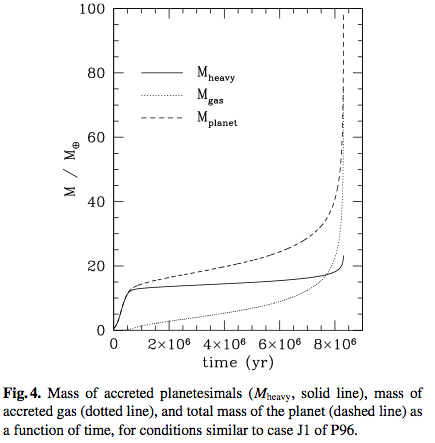
\includegraphics[trim={0cm 2cm 0 0},clip, keepaspectratio,width=0.48\textwidth]{massenvvscore}
\caption{Massa planetaria in funzione della massa del core. Da \cite{alibert2005models}.}\label{fig:massenvvscore}
\end{wrapfigure}

Se il protopianeta raggiunge un valore critico di massa, dipendente debolmente da luminosit\'a generata da accrescimento dei pianetesimi e opacit\'a, per mantenere equilibrio idrostatico l'inviluppo gassoso del pianeta si contrae su tempi scala di Kelvin-Helmholtz. In questa seconda fase l'accresscimento di massa diviene cos\'i rapido da esaurire il gas disponibile nella regione: curva verticale di figura (\ref{fig:massenvvscore}). L'accrescimento di gas has come limite superiore il flusso di gas dovuto a evoluzione viscosa del disco.

Da modelli numerici risulta
\begin{equation}
M_c^{crit}=10\mearth{}(\frac{\dot{M}_c}{\num{e-7}\mearth{}\si{\per\year}})\expy{q}(\frac{\kappa}{\SI{0.1}{\square\meter\per\kilo\gram}})\expy{s}
\end{equation}
con $q,s\approx0.2-0.3$ (\cite{ikoma2000formation}).

\vspace{2cm}

\section{Accrescimento limitato da velocit\'a di raffreddamento}

Seguendo (\cite{mordasini2012characterization}) la struttura del pianeta \'e determinata integrando le equazioni di conservazione di massa, momento e l'equazione del trasporto di energia:
\begin{align}
&\TDy{r}{m}=4\pi r^2\rho\\
%&\TDy{r}{l}=0\\
&\TDy{r}{P}=-\frac{Gm}{r^2}\rho\\
&\TDy{r}{T}=\frac{T}{P}\TDy{r}{P}\nabla(T,P)\\
&\nabla(T,P)=\TDly{P}{T}=\min{(\nad{},\nrad{})}
\end{align}
dove $\nrad{}$ e $\nad{}$ indicano il gradiente radiativo e adiabatico.

La luminosit\'a del pianeta \'e determinata tramite
\begin{equation}
E_t=E_g+E_i=\int_0^M\frac{Gm}{r}\,dm+\int_{M_z}^Mu\,dm=-\xi\frac{GM^2}{2R}
\end{equation}
che sostituita nell'equazione di conservazione dell'energia da:
\begin{equation}
-\TDof{t}E_t=L=L_M+L_R+L_{\xi}=\xi\frac{GM}{R}\dot{M}-\xi\frac{GM^2}{2R^2}\dot{R}+\frac{GM^2}{2R}\dot{\xi}
\end{equation}
con $\dot{M}=\dot{M}_Z+\dot{M}_{XY}$.

Ho indicato la massa di gas legata al core con
\begin{equation}
M_{XY}=4\pi\int_{R_c}^R\rho(r')r'^2\,dr'
\end{equation}
con $R_C$ \'e il raggio del core.

Condizioni al bordo:
\begin{align}
&R=\frac{R_B}{1+R_B/(k_lR_H )},\ P=P_{neb}\\
&\tau=\max{(\rho_{neb}\kappa_{neb}R),2/3)},\ T_i^4=\frac{3\tau L_{int}}{8\pi\sigma R^2}\\
&T^4=T_{neb}^4+T_{int}^4,\ L(R)=L_{int}
\end{align}
$k_{liss}=3-4$, quindi $R_p\approx \min{(R_B,k_{liss}R_H)}$ e introduco il raggio di Bondi
\begin{equation}
R_B=G\frac{M_c}{c_0^2}\approx\SI{4e10}{\cm}a(AU)\expy{1/2}\frac{M_c}{\mearth{}}
\end{equation}
definito come raggio in cui energia termica e potenziale gravitazionale si equivalgono.%il core perturba la pressione del gas del disco.

\begin{workout}[envelope mass as function of core mass]
Armitage 17 eq 232 (`'lecture nite on formation and early evolution of PS)
\begin{equation}
M_{env}\approx\int_{R_c}^{R_o}4\pi r^2\rho\,dr\propto\frac{\sigma}{\kappa_RL}(\frac{\mu m_pGM_t}{4k_b})^4\ln{\frac{R_o}{R_c}}
\end{equation}
\end{workout}

\begin{workout}[Rfes per espressione raggio bondi]

\end{workout}


\begin{workout}[Hydrostatic equilibrium hypothesis]
Characterization of exoplanets from their formation I (eq 10)
\end{workout}


\begin{workout}[Rfes espressione accrescimento gas]
Rate di accrescimento limitato dalla velocit\'a di raffreddamento:
\begin{equation}
\dot{M}_{XY}\propto\ \frac{M_p}{M_*}<(H_P/R_p)^3/\sqrt{3}
\end{equation}
quindi la massa di gas aumenta esponenzialmente a partire da $M_c\approx10\mearth{}$.
\end{workout}

\section{Accrescimento limitato dalla disponibilit\'a di gas del disco}

Se $H\approx R$ il pianeta perturba in maniera non trascurabile il disco (il rate di accrescimento di gas \'e maggiore di quello fornito dal disco). Il raggio del pianeta \'e determinato dalle condizioni al bordo per materia accresciuta tramite free-fall da $R_H$ a $R$:
\begin{align}
&\dot{M}_{XY}=\dot{M}_{XY,max},\ v_{ff}^2=2GM(\frac{1}{R}-\frac{1}{R_H})\\
&P=P_{neb}+\frac{\dot{M}_{XY}}{4\pi r^2}v_{ff}+\frac{2g}{3\kappa},\ \tau=\max{(\rho_{neb}\kappa_{neb}R,2/3)}\\
&T_{int}^4=\frac{3\tau L_{int}}{8\pi\sigma R^2},\ T^4=(1-A)T_{neb}^4+T_{int}^4
\end{align}

In questa fase la velocit\'a di accrescimento di gas \'e determinata dall'evoluzione viscosa del disco:
\begin{equation}
\dot{M}_{e,visc}=f_{hyd}3\pi\nu\Sigma_g
\end{equation}
$f_{hyd}\approx0.9$ valore determinato da simulazioni idrodinamiche (\cite{lubow1999disk}).

\begin{workout}[Bondi accretion rate]
Unperturbed viscous flow
\begin{equation}
\dot{M}_{e,B}\approx\frac{\Sigma_g}{H}(\frac{R_H}{3})^3\Omega
\end{equation}
\end{workout}

\begin{workout}[Detached phase accretion rate]
Characterization of exoplanets from their formation pg 8
\end{workout}

\begin{workout}[Wien displacement]
$\lambda_{max}T\approx \SI{3e-3}{\meter\kelvin}$
\end{workout}

\begin{workout}[Critical core mass]
From toward deterministic
\begin{equation}
M_{c,crit}\approx10(\frac{\dot{M}_c}{\num{e-6}\mearth{}\si{\per\year}})\expy{0.2-0.3}(\frac{\kappa}{\SI{1}{\square\cm\per\gram}})\expy{0.2-0.3}\mearth{}
\end{equation}•
\end{workout}

\begin{workout}[gas accretion refs]
Lissauer 09: Models of Jupiter’s growth incorporating thermal and hydrodynamic constraints
Rafikov 10: ''Constraint on giant planet production by core accretion''
Rafikov 04 Atmospheres of protoplanetary cores: critical mass for nucleated instability.
Refs: Planet formation models: the interplay with the planetesimal disc (Fortier 2013), Characterization of exoplanets from their formation I. Models of combined planet formation and evolution (Mordasini 12)
\end{workout}

\begin{workout}[Planet-Disk exchange in hydrodynamic manner]
Ormel 15/ Cimerman 17
\end{workout}

%\section{Fase isolata}

\begin{workout}[Fase isolata: fonti energia]
fonti energia: tidal heating radiogeninc heat, star flux
\end{workout}


{\let\clearpage\relax\let\cleardoublepage\relax
\chapter{Evoluzione orbite proto-pianeti: migrazione planetaria.}
}

L'osservazione di una sottopopolazione di esopianeti giganti su orbite strette, per cui sembra improbabile una formazione in loco, e la presenza di sistemi multipli in risonanza sono indicatori di evoluzione orbitale, d'altra parte nel Sistema solare fenomeni di migrazione fornisco una spiegazione all'orbita di plutone, alla presenza di numerosi oggetti della fascia di Kuiper in risonanza $3:2$ con Nettuno e al periodo di collisioni intense testimoniato da craterizzazione (Late heavy bombardment).

Fenomeni che possono dar luogo a migrazione planetaria:
\begin{itemize}
\item Interazione con disco proto-planetario. Elenco schematicamente alcuni risultati da \cite{armitage2007lecture} e \cite{crida2006planetary}.
Considerando le perturbazioni lineari nella densit\'a del disco prodotte dal potenziale del pianeta si determina la risultante dei momenti torcenti $\Gamma$ dovuti alle risonanze di Lindblad e alla regione di corotazione. La migrazione di tipo I ha tempi caratteristici
\begin{equation}
\tau_I\propto\frac{M_p}{\Gamma}\propto M_p\expy{-1}
\end{equation}
per pianeta $5\mearth{}$ a \SI{5}{\astronomicalunit} si ha $\tau_I=\SI{0.5}{\mega\year}$.

La migrazione di tipo II \'e caratterizzata da formazione di un gap attorno all'orbita del pianeta: la transizione tra migrazione I e II avviene se $R_H>H$ e momento torcente dovuto alla viscosit\'a del disco \'e minore del momento esercitato dal pianeta sul disco. La velocit\'a di migrazione di tipo II \'e determinata dall'evoluzione viscosa del disco:
\begin{equation}
\dot{a}_p=-\frac{3}{2}\frac{\nu}{r}
\end{equation}
Il momento esercitato sul pianeta dalla regione di corotazione pu\'o dar luogo a feedback positivo su pianeta di massa intermedia con velocit\'a radiale $\dot{a}_p$.

\item Interazione con disco residuo di planetesimi

\item Interazione tra due o pi\'u pianeti giganti

\item Interazione con stella in sistema di stelle binarie

\item Interazione mareale con la stella

\end{itemize}

%{\let\clearpage\relax\let\cleardoublepage\relax
%\chapter{N-body interactions inside proto disk}
%}


\begin{workout}[Long-term evolution: laplace equations]
The HARPS search for southern extra-solar planets-XXVIII. Up to seven planets orbiting HD 10180: probing the architecture of low-mass planetary systems
\end{workout}
